\documentclass[11pt,oneside,letterpaper]{article}

% graphicx package, useful for including eps and pdf graphics
\usepackage{graphicx}
\DeclareGraphicsExtensions{.pdf,.png,.jpg}

% basic packages
\usepackage{color}
\usepackage{parskip}
\usepackage{float}

% text layout
\usepackage{geometry}
\geometry{textwidth=15cm} % 15.25cm for single-space, 16.25cm for double-space
\geometry{textheight=22cm} % 22cm for single-space, 22.5cm for double-space

% helps to keep figures from being orphaned on a page by themselves
\renewcommand{\topfraction}{0.85}
\renewcommand{\textfraction}{0.1}

% bold the 'Figure #' in the caption and separate it with a period
% Captions will be left justified
\usepackage[labelfont=bf,labelsep=period,font=small]{caption}

% review layout with double-spacing
%\usepackage{setspace}
%\doublespacing
%\captionsetup{labelfont=bf,labelsep=period,font=doublespacing}

% cite package, to clean up citations in the main text. Do not remove.
\usepackage{cite}
%\renewcommand\citeleft{(}
%\renewcommand\citeright{)}
%\renewcommand\citeform[1]{\textsl{#1}}

% Remove brackets from numbering in list of References
\renewcommand\refname{\large References}
\makeatletter
\renewcommand{\@biblabel}[1]{\quad#1.}
\makeatother

\usepackage{authblk}
\renewcommand\Authands{ \& }
\renewcommand\Authfont{\normalsize \bf}
\renewcommand\Affilfont{\small \normalfont}
\makeatletter
\renewcommand\AB@affilsepx{, \protect\Affilfont}
\makeatother

% notation
\usepackage{amsmath}
\usepackage{amssymb}

%%% TITLE %%%
\title{\vspace{1.0cm} \Large \bf
ncov-forecasting-fit (title TBD)
}

\author[1,2]{Eslam Abousamra}
\author[1,3]{Marlin Figgins}
\author[1,2,4]{Trevor Bedford}

\affil[1]{Vaccine and Infectious Disease Division, Fred Hutchinson Cancer Center, Seattle, WA, USA}
\affil[2]{Department of Epidemiology, University of Washington, Seattle, WA, USA}
\affil[3]{Department of Applied Mathematics, University of Washington, Seattle, WA, USA}
\affil[4]{Howard Hughes Medical Institute, Seattle, WA, USA}

\date{}

\begin{document}

\maketitle

%%% ABSTRACT %%%
\begin{abstract}

Todo

\end{abstract}

%%% INTRODUCTION %%%
\section*{Introduction}

I use Google Scholar format for citation style with first author, year and first word of title, ala \cite{hadfield2018nextstrain}.

%%% METHODS %%%
\section*{Methods}

Todo

%%% RESULTS %%%
\section*{Results}

I put figures into a `/figures' directory and use semantic labeling ala (Figure~\ref{example_predictions}).

%%% map %%%
\begin{figure}[h]
	\centering
	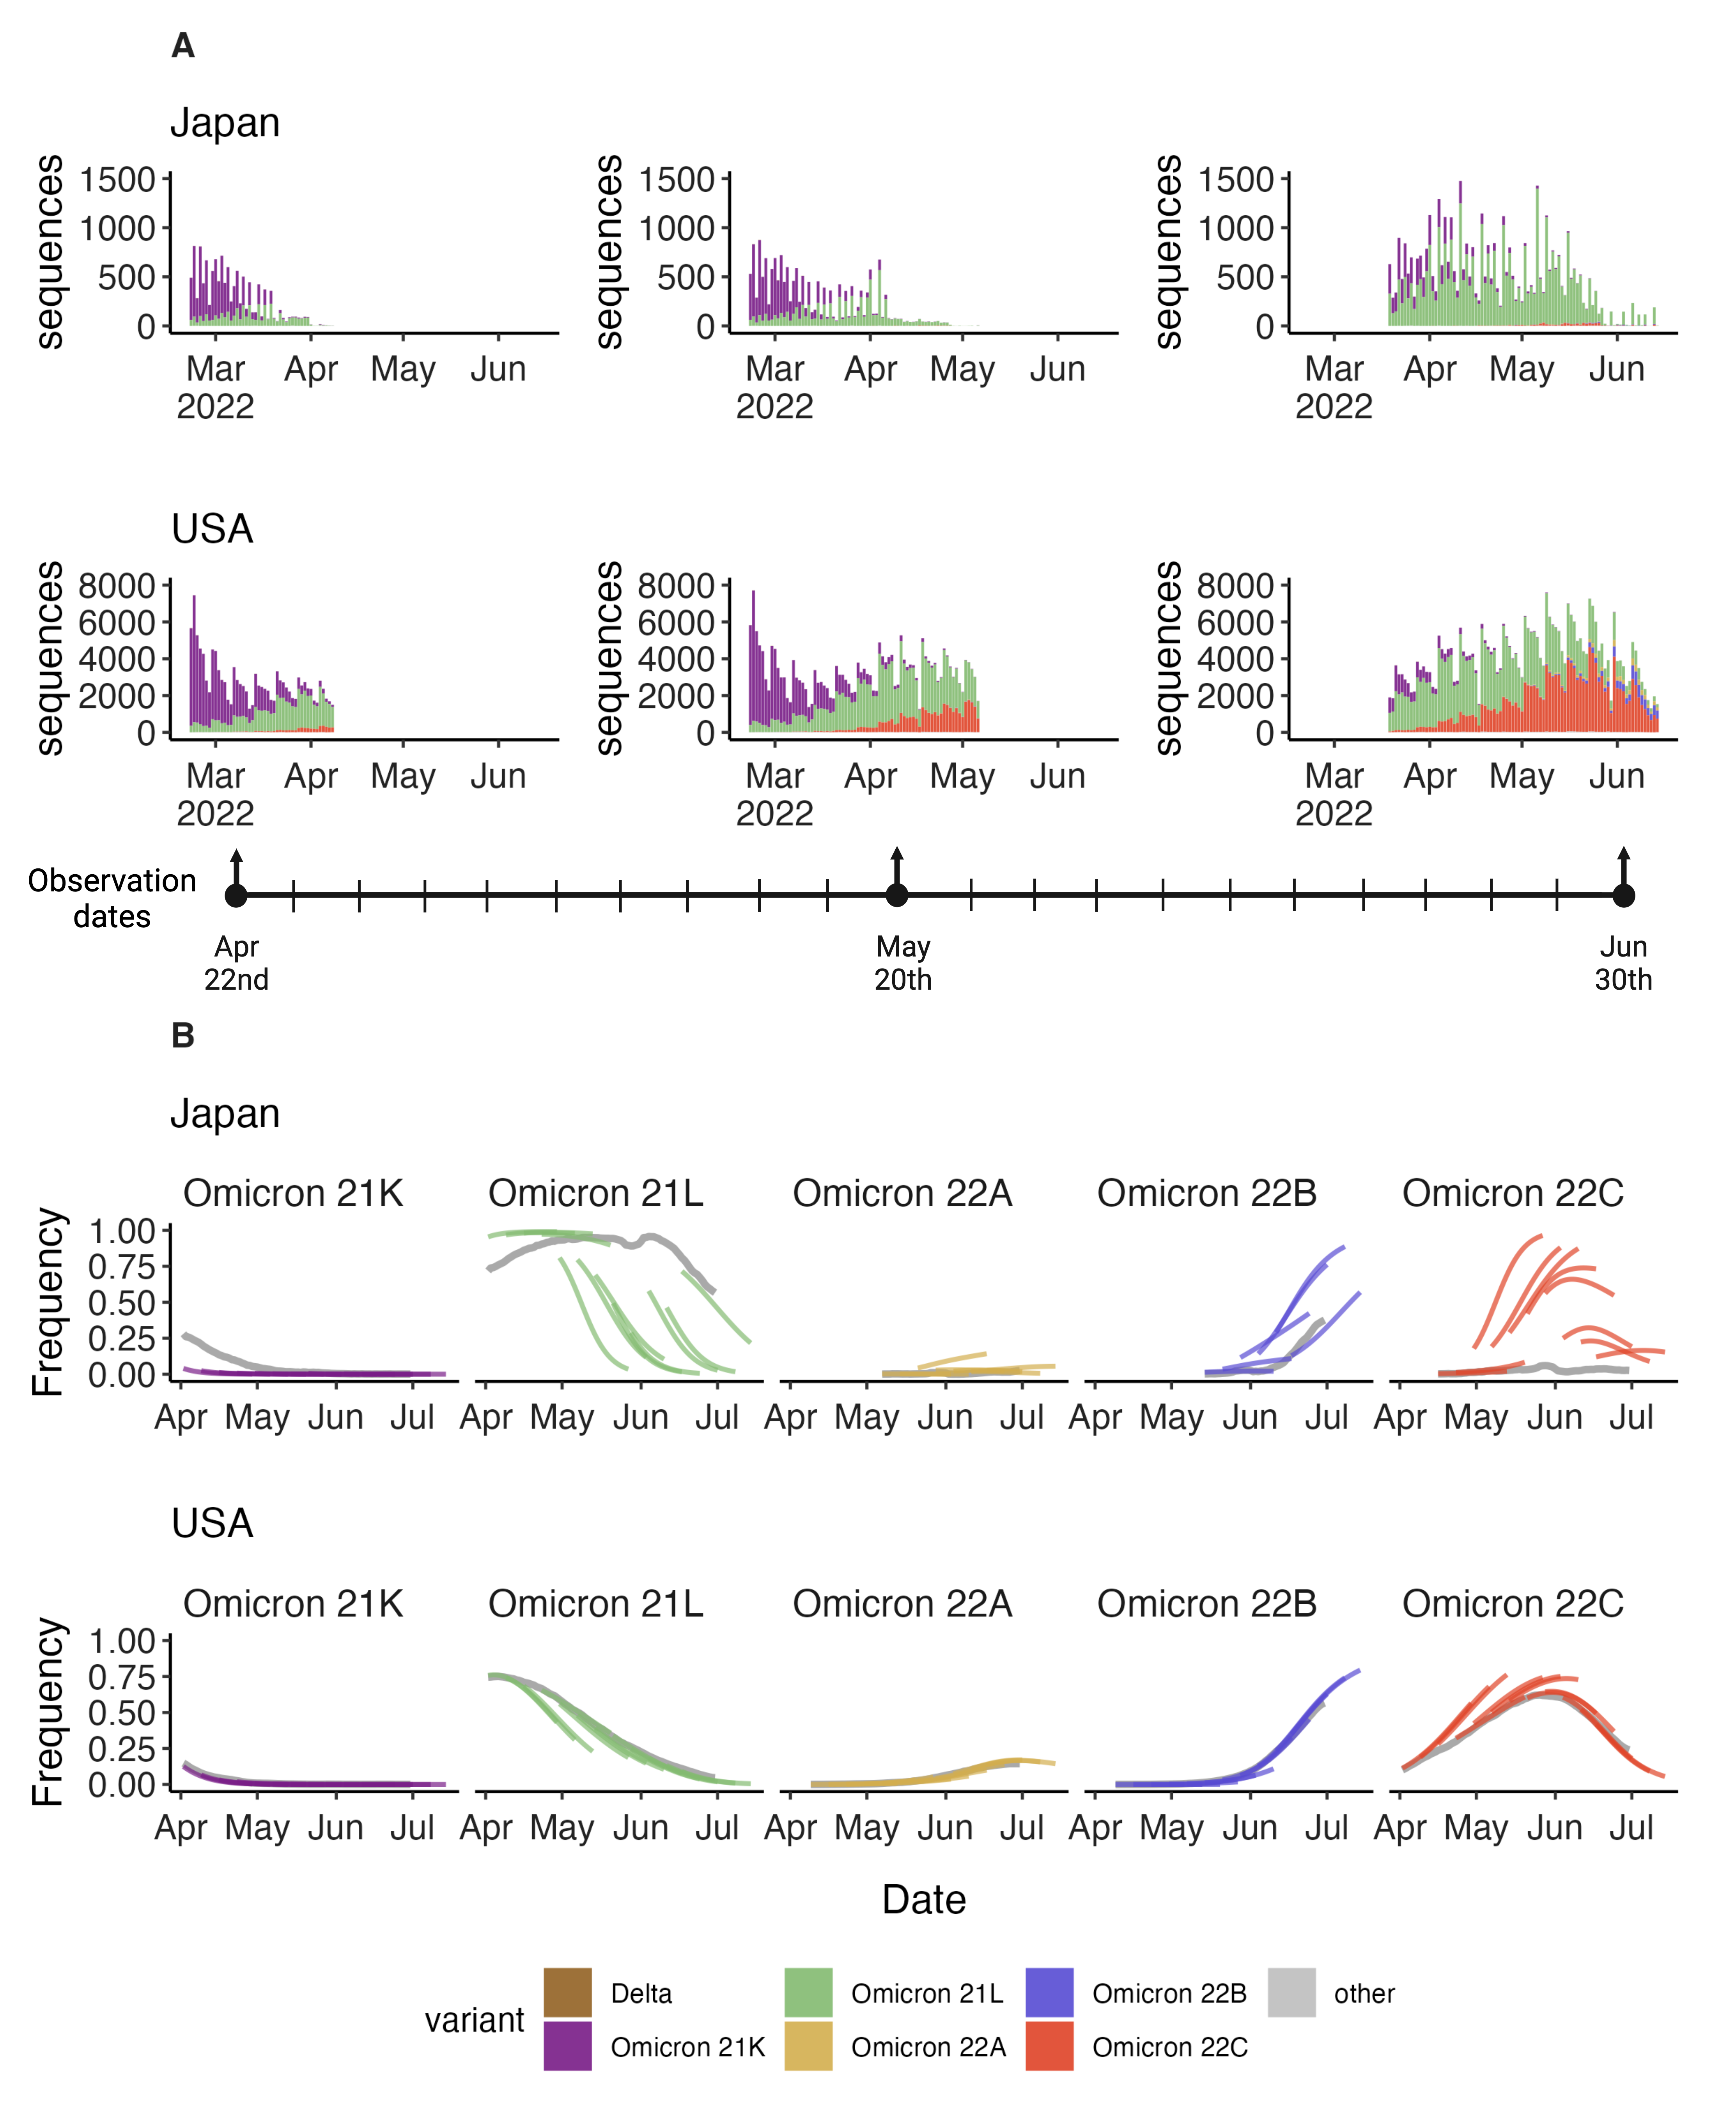
\includegraphics[width=1.0\textwidth]{figures/example_predictions}
	\caption{\textbf{Example data and predictions for Japan and the USA.}
	Further legend here.
	}
	\label{example_predictions}
\end{figure}

%%% DISCUSSION %%%
\section*{Discussion}

Todo

%%% REFERENCES %%%
\bibliographystyle{plos}
\bibliography{ncov-forecasting-fit}

\end{document}
